\chapter{Introdução}\label{introducao}
% determinacao da potencia sonora
Várias técnicas de controle de ruído foram desenvolvidas nesses últimos tempos visando oferecer ao ouvido humano um ambiente agradável, principalmente em ambientes de salas nas quais aspecto reverberante é bastante evidente.

Com esse determinado fim, o uso de materiais de absorção de ondas sonoras é amplamente utilizado. Esses materiais, normalmente porosos, ficam nas extremidades de uma sala reverberante amortecendo e dissipando em forma de energia térmica o som. Em vista desse aspecto todo material que visa esse objetivo possui um coeficiente de absorção sonora e o mesmo é levado em consideração para o controle de ruído numa sala por exemplo.

Em vista do que foi exposto, esse trabalho tem como objetivo analisar o coeficiente de absorção sonora de uma amostra de um material poroso através da câmara de reverberação. Para isso, utilizou-se
como base a norma ISO 354:2003, que estabelece os procedimentos que devem ser feitos para
determinar tal parâmetro em uma câmara reverberante

\chapter{Fundamentação Teórica}\label{fundamentacao}
% Som
Em vista do que se expõe em \cite{bistafa}, o som é a aceleração de partículas de ar que se chocam, transformando a pressão estática do ar numa pressão oscilatória. Essa pressão oscilatória entre em contato com os ouvidos do ouvinte fazendo com que essa variação de pressão seja percebida e escutada. Essa variação de pressão que oscila é escutada pelo ser humano a partir da magnitude de pressão de $2\cdot10^{-5}$ $Pa$. Qualquer pertubação de pressão que se encaixa nessas condições é denominada som e as pertubações indesejáveis são denominadas de ruído sonoro.

Para se mensurar o nível de pressão sonora deve-se comparar	o valor $rms$ da pressão coletada pela pressão de referência ($2\cdot10^{-5}$ $Pa$), usando a operação de divisão. Como a magnitude dessa divisão é muita alta, a variação das pressões audíveis é de ordem muito alta fazendo assim que se transforme esse valor numa medida logarítmica e multiplicado por 10. A expressão matemática resultante desse processo é 
\begin{equation}
  NPS  = 10 . log_10(p_{rms}^{2}/(2\cdot10^{-5})^{2}).
\end{equation}
Tal que $NPS$ é o nível de pressão sonora e $p_{rms}$ é o $rms$ da pressão coletada.
% pressao sonora

% potencia
De acordo com \cite{potencia}, a potência sonora é uma grandeza física que diz respeito à energia acústica total emitida por uma determinada fonte sonora. Dessa forma, a potência sonora depende apenas da própria fonte e independe das características do meio, fazendo com que esse tipo de grandeza física se qualifique como satisfatório para caracterizar uma fonte sonora. Em vista disso a potência sonora é dada pela equação
\begin{equation}
W = I_{max}S.
\label{eq.potencia}
\end{equation}
Tal que $W$ é a potência sonora, $I_{max}$ intensidade sonora máxima e $S$ é a área. Como a intensidade sonora máxima ($I_{max}$) se relaciona com a impedância característica do meio ($\rho . c$) de tal forma que a expressão matemática de denota como \begin{equation}
I_{max}=\frac{p_{rms}^{2}}{\rho_{0} . c}.
\label{eq.intensidade}
\end{equation}
Dessa forma, dividindo por uma potência de referência $W_{o}= \frac{p_{o}^{2}}{\rho c}S $ a equação da potência pode ser caracterizada por
 \begin{equation}
	\frac{W}{W_{o}}=\frac{p_{rms}^{2}}{p_{o}^{2}}\frac{S}{S_{o}}.
\label{eq.relpotencia}
\end{equation}
Aplicando a operação logarítmica na equação \ref{eq.relpotencia} o resultado final do cálculo da potência é
\begin{equation}
	NWS = NPS + 10 . log_{10}\left(\frac{S}{S_{o}}\right).
\end{equation}

% calculo potencia anecoicaa
Para se medir a potência sonora há ambientes apropriados que são as câmaras anecóicas e câmaras reverberantes. As câmaras anecóicas, são construídas com superfícies configuradas para absorver toda a energia sonora incidente, simulando um campo livre com reflexões anuladas nas paredes. No extremo oposto, as câmaras reverberantes são construídas de tal forma a maximizar o som refletido pelas paredes, no sentido de gerar campo difuso.

Para medir a pressão sonora nas câmaras anecóicas deve-se usar os microfones de campo livre nos quais são projetados de forma direcional para a fonte sonora. Essa caracterísca faz a onda incidir de forma longitudinal no microfone. Para se medir a pressão sonora nas câmaras reverberantes deve-se usar os microfones de campo difuso nos quais são projetados de forma que as ondas se incidem em todos os lados desse tipo de microfone.


O tempo de reverberação é postulado o intervalo de tempo em segundos que a densidade de energia sonora demora para decair numa escala de 60 dB. Quando uma fonte gera som dentro de uma sala, a intensidade sonora cresce rapidamente com a chegada do som direto e continuará crescendo com as reflexões indiretas que começam a contribuir para o nível sonoro total. Se uma fonte sonora é repentinamente desligada, a intensidade sonora não desaparecerá de repente, mas vai enfraquecendo gradualmente. Este decaimento de energia sonora ocorre em função da forma da sala e a quantidade e localização dos materiais absorventes, e é conhecido como reverberação.

Há duas formas de se determinar o tempo de reverberação que são a forma de Sabine e a forma de Eyring. A forma de Sabine é definida como:
\begin{equation}
	T_{r}= 0,161 . \frac{V}{S . \alpha}.
\label{eq.relpotencia}
\end{equation}

Já a forma de Eyring é definida como:
\begin{equation}
	T_{r}= 0,161 . \frac{V}{S . ln (1 - \alpha)}.
\label{eq.relpotencia}
\end{equation}

Tais quais $T_{r}$ é o tempo de reverberação em segundos, $\alpha$  é o coeficiente de absorção, $V$ é o volume do ambiente em metros cúbicos e $S$ é a área total superficial da sala.

\chapter{Experimento e Equipamentos}\label{descricao}

% instrumentos de medicao
Para realizar as medições tais instrumentos foram utilizados:
\begin{itemize}
	\item Microfone capacitivo de campo livre:
		\begin{itemize}
			\item Tipo número 4189-A-021;
			\item Sensibilidade -26.7 dB re 1V/Pa;
			\item Incerteza, 95\% de nível de confiança de 0.2 dB.
		\end{itemize}
	\item Microfone capacitivo de campo difuso:
		\begin{itemize}
			\item Tipo número 4942-A-021;
			\item Sensibilidade -26.3 dB re 1V/Pa;
			\item Incerteza, 95\% de nível de confiança de 0.2 dB.
		\end{itemize}
	\item Calibrador de microfone tipo CAL 200, da Larson Davis. Nível de calibração 94/114 dB;
	\item Fonte sonora tipo 4204:
		\begin{itemize}
			\item Cumpre ISO 3741 , ISO 3747 e ISO 6926 para calibrar fontes de potência sonora;
			\item Gama de frequências de 100 Hz a 20 kHz;
			\item Saída de potência sonora 91 dB re 1 pW (peso A, freqüência de linha de 50 Hz) e 95 dB re 1 pW (Aweighted , freqüência de linha de 60 Hz);
			\item Gama de temperaturas de -10ºC a + 50ºC;
			\item Operação 50 e 60 Hz.
		\end{itemize}
	\item Tripé e Cabos;
	\item Analisador de sinais modelo SCADAS da LMS:
	\begin{itemize}
		\item módulo de condicionamento e aquisição (com 4 ou 8 canais dinâmicos) com frequência de amostragem de 102,4 KHz e 24 bits de resolução;
		\item duas entradas para tacómetro com taxas de amostragem de até 6,5 MHz;
		\item dois geradores de função.
	\end{itemize}
	\item Rotating boom tipo 3923:
		\begin{itemize}
			\item Cumpre ISO 3741;
			\item Comprimento da lança ajustável entre 50 cm e 200 cm;
			\item Operação com bateria com células NiCd ou operação de linha embutidos;
			\item Três vezes rotação do interruptor selecionável;
			\item Plano de rotação ajustável em passos de 10 graus;
			\item E poder de sinal do microfone via anéis deslizantes;
			\item Potência sonora emitida típico igual a 26 dB re 1 pW (peso A).
		\end{itemize}

	\item Material de absorção do tipo Espuma Sonex: 
		\begin{itemize}
			\item Os painéis Sonex ValueLine oferecem excelente controle acústico em todas as frequências com coeficientes de redução (NRC), variando de 0,75 a 1,05;
			\item Eles são especialmente eficazes em absorção excessiva nas freqüências médias (500 e 1.000 Hz);
			\item Neste ensaio foi utilizada uma amostra de material de absorção com 8,64 $m^{2}$.
		\end{itemize}

	Para medição do tempo de reverberação na câmara reverberante foram seguidos os procedimentos descritos na ISO 354 Measurement of sound absorption in a reverberation room. Foram feitas medições com e sem o material de absorção analisado, sendo utilizados 3 microfones para as medições, variando 3 posições de fonte sonora.

	Foi analisada a faixa de frequência de 63 Hz a 10000 Hz. Para determinar o tempo de reverberação foi utilizada a equação 06 descrita na ISO 354. A técnica de medição utilizada foi a do ruído interrompido, onde foram feitas 3 médias para cada tomada de dados de tempo de reverberação, sendo enviado um sinal de ruído branco na sala. Para se determinar o coeficiente de absorção utilizou-se a fórmula $\alpha = A_{t}/S$, tal qual $\alpha$ é o coeficiente de absorção, $A_{t}$ é a área de absorção equivalente e $S$ é a área da amostra.		

\end{itemize}

\chapter{Resultados}\label{resultados}

\section{Tempo de Reverberação} % (fold)

É possível observar a nítida influência do material de absorção principalmente a partir da faixa de frequência de 400 Hz sendo possível verificar uma diferença de 2 segundos em relação aos resultados obtidos com a sala vazia, como é mostrado no gráfico \ref{figura_1}.

\begin{figure}[h!]
    \centering
    %\hspace{-4.5cm}
    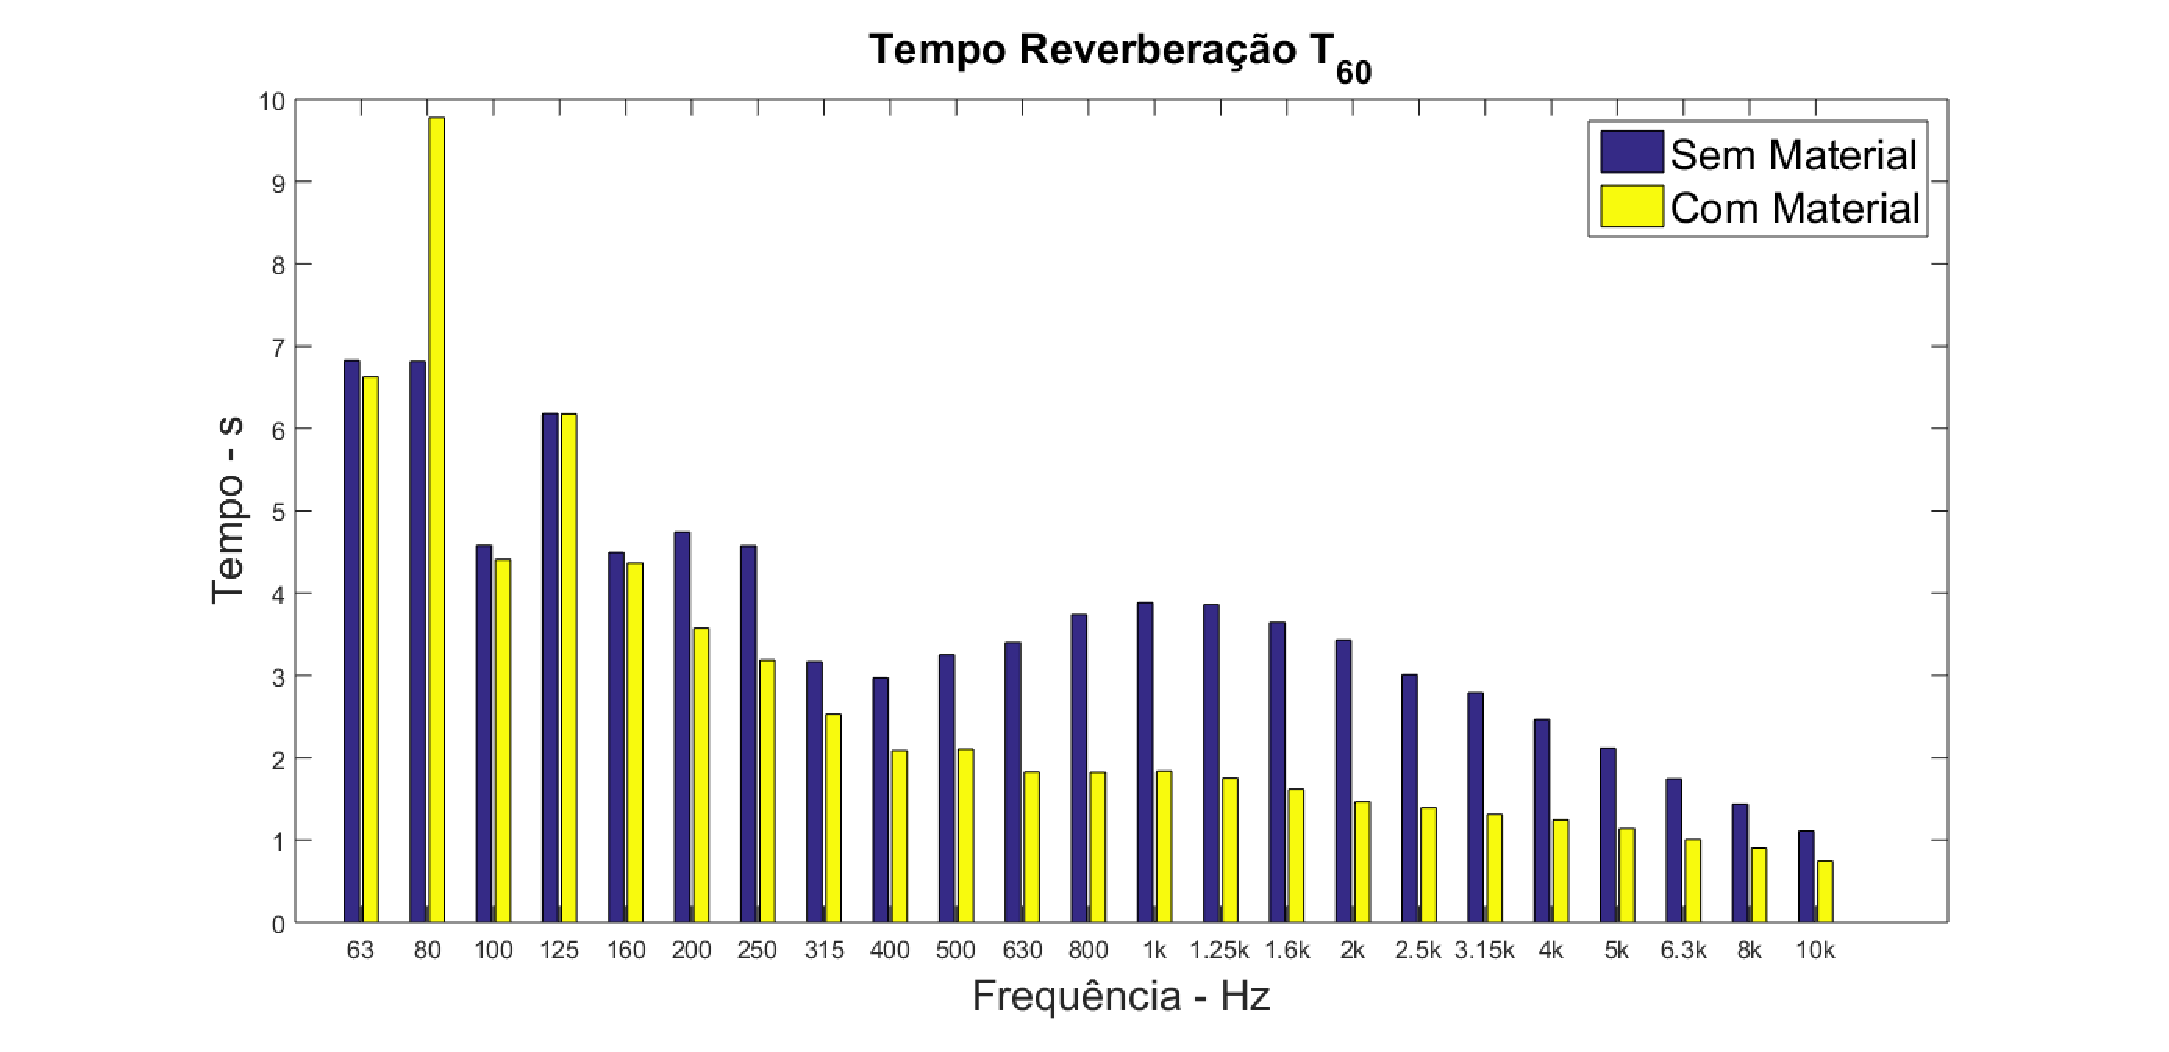
\includegraphics[width=1.2\textwidth]{imagem1.eps}
    \caption{Tempo de reverberação na sala. Fonte: autoria própria.}
    \label{figura_1}
\end{figure}

Ao analisar o gráfico \ref{figura_2} é possível observar a variação coerente do coeficiente de absorção sonora, crescendo para as altas frequências e ficando abaixo do valor de 1, ou seja, $100\%$ de absorção. É importante ressaltar que a faixa de interesse desta medição é acima da frequência de corte e abaixo do valor em alta frequência aonde a sala apresenta divergências.

\section{Coeficiente de Absorção}
\begin{figure}[h!]
    \centering
    %\hspace{-4.5cm}
    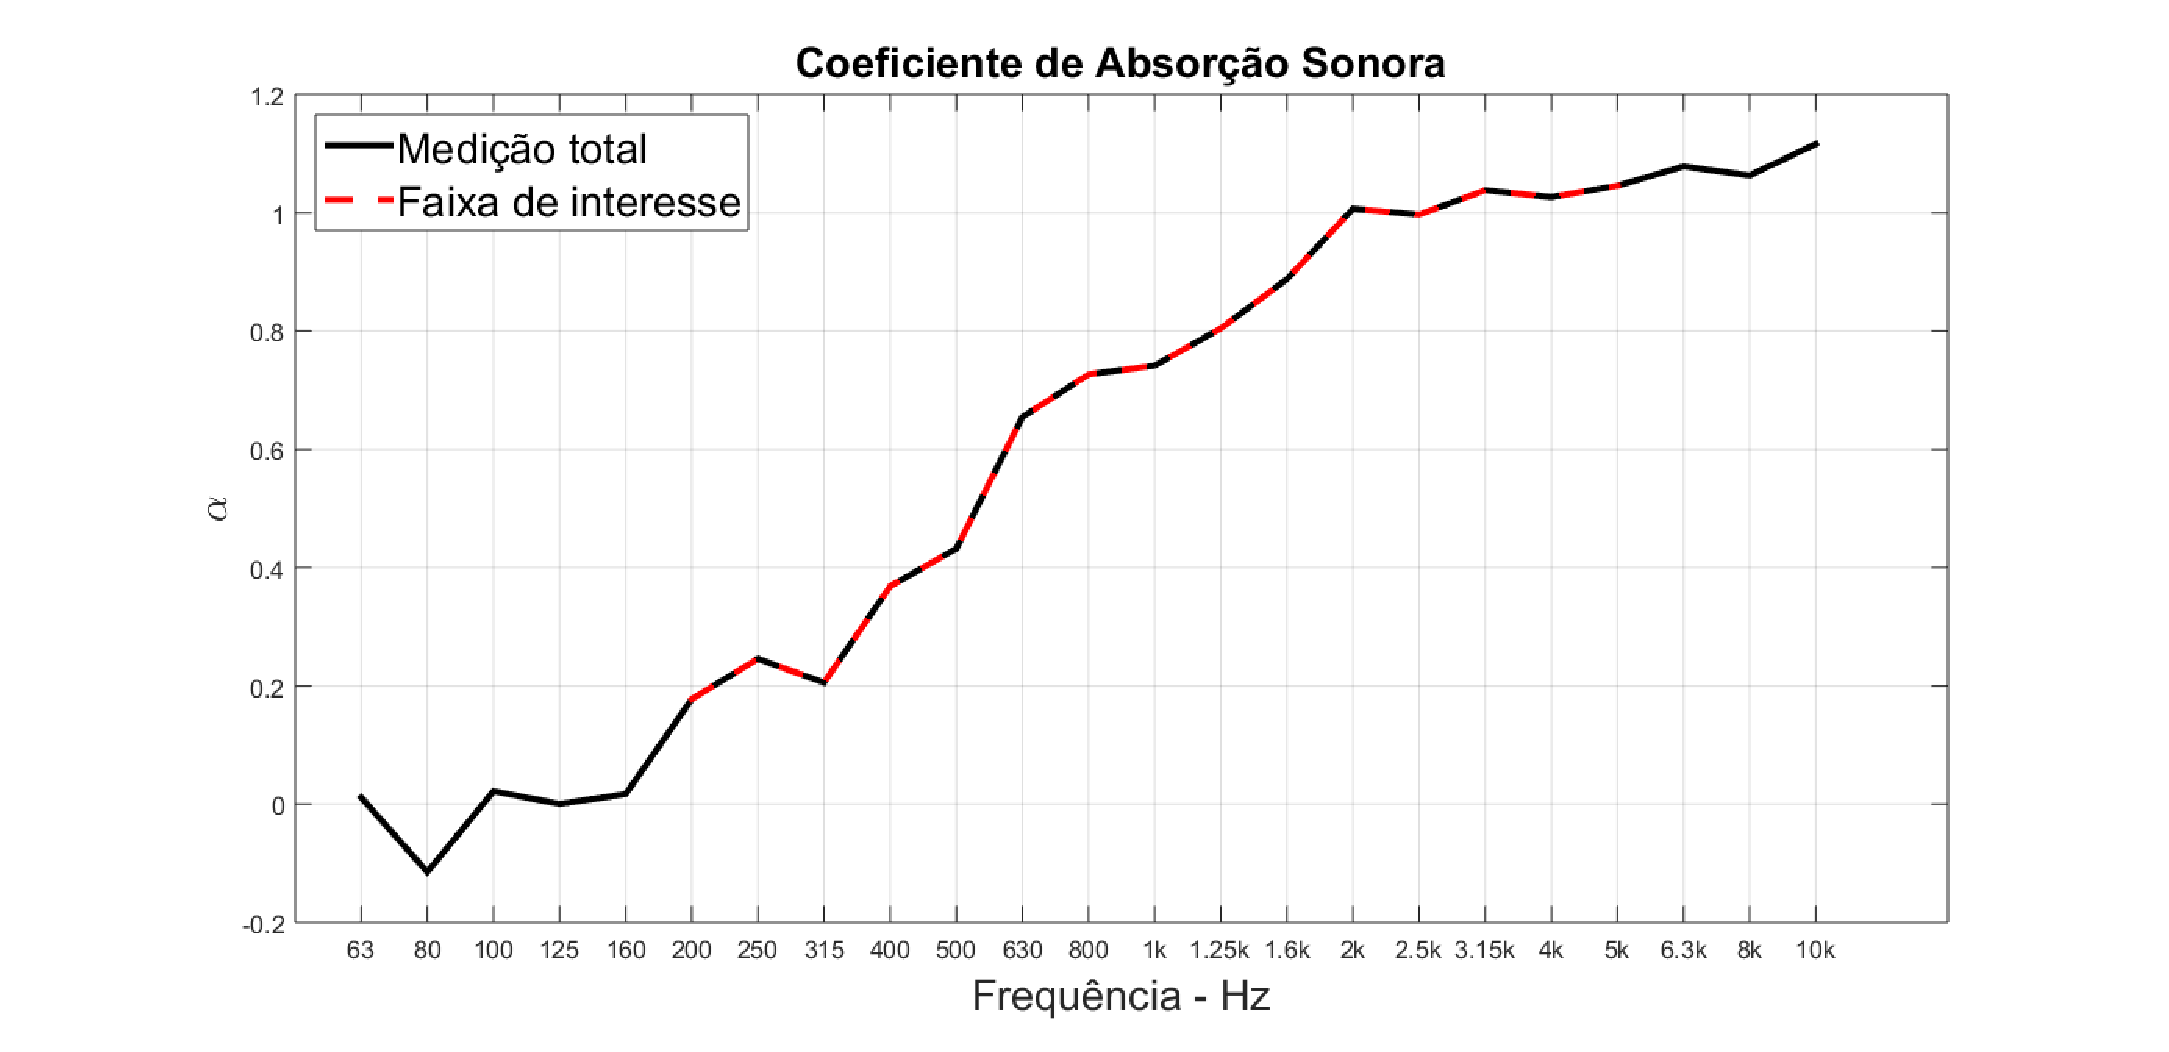
\includegraphics[width=1.2\textwidth]{imagem2.eps}
    \caption{Coeficiente de absorção sonora do material. Fonte: autoria própria.}
    \label{figura_2}
\end{figure}


\chapter{Conclusões}\label{conclusoes}

Em vista do que foi apresentado, a realização dos ensaios na câmara reverberante originou resultados que constam de acordo com a teoria vigente visto que o tempo de reverberação decai pela metade com a inserção do material poroso dentro do ambiente, e esse fato se intensifica quando a análise é feita nas altas frequências pois é nessa mesma faixa de frequência que as moléculas do ar se agitam rapidamente, aumentando, assim, a quantidade de colisões no material absorvente.
